% Master thesis — Uncertainty-Aware Diabetic Retinopathy Grading
% Compile: pdflatex main && bibtex main && pdflatex main && pdflatex main
%
% This is a skeleton. Fill the chapter \input{} stubs with prose; tables
% and figures are auto-generated and live under thesis/{tables,figures}.

\documentclass[12pt,a4paper,oneside]{report}

\usepackage[utf8]{inputenc}
\usepackage[T1]{fontenc}
\usepackage[english]{babel}
\usepackage{lmodern}
\usepackage{microtype}

% Math + tables + figures
\usepackage{amsmath, amssymb}
\usepackage{booktabs}
\usepackage{graphicx}
\usepackage{caption}
\usepackage{subcaption}
\usepackage{float}
\usepackage{array}

% Bibliography
\usepackage[backend=biber,style=ieee,sorting=nyt]{biblatex}
\addbibresource{references.bib}

% Code listings
\usepackage{listings}
\usepackage{xcolor}
\lstset{
  basicstyle=\ttfamily\footnotesize,
  keywordstyle=\color{blue!70!black},
  commentstyle=\color{green!50!black}\itshape,
  stringstyle=\color{red!60!black},
  frame=single,
  rulecolor=\color{gray!40},
  breaklines=true,
  showstringspaces=false,
}

\usepackage[hidelinks]{hyperref}
\usepackage[capitalize]{cleveref}

\title{Uncertainty-Aware Diabetic Retinopathy Grading via Conformal Prediction
       and Bayesian Deep Learning}
\author{Alketa Alia}
\date{\today}

\begin{document}

\maketitle

\begin{abstract}
% Abstract — ~250 words.
Diabetic retinopathy (DR) is a leading cause of preventable blindness, and
automated screening systems are expected to scale early detection. While
recent deep-learning models for DR classification report high accuracies,
clinical deployment is hindered by their tendency to produce
\emph{over-confident} predictions: when a model is wrong, it is often
just as confident as when it is right.

This thesis builds an \emph{uncertainty-aware} DR grading system on top of
the APTOS~2019 fundus dataset. Six baseline architectures (ResNet50,
DenseNet121, VGG16, Xception, a custom CNN, and a CNN with mixed
\textit{tanh}+\textit{ReLU} activations) are first evaluated as binary
classifiers using a stratified 70/15/15 split. With proper preprocessing
and class weighting, all five strong baselines reach 95--96\,\%
test accuracy, which McNemar tests show is statistically indistinguishable
across them. A heterogeneous ensemble pushes accuracy to 96.55\,\% and
predictive entropy enables \emph{selective prediction} that reaches
99.6\,\% accuracy at 50\,\% coverage.

We then add three uncertainty-aware components: (i) split conformal
prediction with formal coverage guarantees at $\alpha = 0.10$ and
$\alpha = 0.05$; (ii) Monte Carlo Dropout retrained variants of the CNN
and ResNet50; and (iii) multi-method out-of-distribution detection in
which feature-space methods (Mahalanobis, cosine) achieve perfect
separation against synthetic OOD inputs. Five-fold cross-validation
on ResNet50 gives a tight test accuracy of $95.64 \pm 0.18$\,\%, ruling out
single-split luck.

Finally, we re-formulate the task as the clinically meaningful 5-stage
grading scale (No DR, Mild, Moderate, Severe, PDR). The ResNet50
multi-class model achieves a quadratic-weighted kappa of 0.847,
competitive with public APTOS~2019 leaderboards. Combined with conformal
prediction at 90\,\% coverage, the system produces interpretable
prediction sets and a principled clinical refer-to-specialist rule.

\end{abstract}

\tableofcontents
\listoftables
\listoffigures

\chapter{Introduction}
\label{ch:introduction}

% ~6-10 pages

\section{Clinical motivation}
% Outline:
% - DR prevalence (mention WHO numbers, global blindness statistics)
% - 5-stage severity scale and its treatment implications:
%   * No DR / Mild — observation
%   * Moderate — closer follow-up
%   * Severe / PDR — urgent referral, possible laser/anti-VEGF
% - Cost and shortage of trained ophthalmologists, especially in
%   primary care; need for automated triage.

\section{Why uncertainty matters in medical AI}
% Outline:
% - Modern CNNs are over-confident: a wrong 99\%-confident prediction is
%   indistinguishable from a right one.
% - Risk of harm: an overconfident "No DR" can delay vision-saving care.
% - Recent regulatory push (FDA AI-as-a-medical-device, EU AI Act)
%   explicitly requires transparency around model uncertainty.
% - Clinically useful systems should produce a "refer to specialist"
%   recommendation rather than a forced binary verdict on hard cases.

\section{Bachelor recap and research gap}
% Outline:
% - Briefly describe the bachelor thesis (binary classification, 9
%   algorithms, single 80/20 split, accuracy as the only metric).
% - Identify the gaps the master must close:
%   * Multi-class severity grading, not just binary
%   * Statistical significance and confidence intervals
%   * Calibration, not just accuracy
%   * Distribution-free uncertainty guarantees
%   * Out-of-distribution detection
%   * Reproducibility under cross-validation

\section{Contributions}
% Outline:
% 1. A reproducible, statistically rigorous evaluation pipeline for the
%    APTOS 2019 dataset (stratified splits, K-fold CV, McNemar testing).
% 2. Calibration analysis (ECE, MCE, temperature scaling) for six DL
%    architectures, exposing previously unreported over-confidence.
% 3. Application of split conformal prediction (LAC + APS) to DR
%    classification with formal $1-\alpha$ coverage guarantees.
% 4. Comparison of Monte Carlo Dropout, deep-ensemble, and feature-space
%    OOD detection methods on the same test set.
% 5. A 5-stage grading model achieving $\text{QWK} = 0.847$, competitive
%    with the APTOS 2019 Kaggle leaderboard.
% 6. An open-source Streamlit application that surfaces uncertainty
%    visually for end users.

\section{Thesis structure}
% \cref{ch:background} surveys clinical and technical background;
% \cref{ch:methodology} describes the data, splits and shared experimental
% protocol; \cref{ch:phase1} reports binary baselines and calibration;
% \cref{ch:phase2} introduces conformal prediction, OOD detection,
% MC Dropout and K-fold CV; \cref{ch:phase3} extends the system to
% multi-class severity grading; \cref{ch:discussion} discusses clinical
% implications, limitations and future work.

\chapter{Background}
\label{ch:background}

% ~10-15 pages

\section{Diabetic retinopathy and the APTOS 2019 grading scale}
% - Pathophysiology overview (microaneurysms, hemorrhages, neovascularisation).
% - International Clinical DR Severity Scale: No DR (0), Mild (1),
%   Moderate (2), Severe (3), PDR (4).
% - APTOS 2019 dataset description: 3,662 fundus images, 224x224, labelled by
%   one or more ophthalmologists per the above scale.
% - Class imbalance figures (about half are class 0).

\section{Convolutional architectures used}
% - ResNet50, DenseNet121, Xception, VGG16 — short summaries.
% - Transfer learning vs from-scratch CNN: parameter counts,
%   ImageNet pretraining intuition.
% - Why these architectures were chosen (alignment with bachelor study
%   and APTOS literature).

\section{Calibration of deep classifiers}
% - Definition of calibration: $P(\hat y = y \mid \hat p = p) = p$.
% - Empirical calibration error (ECE), maximum calibration error (MCE),
%   reliability diagrams (\citealp{guo2017calibration,naeini2015obtaining}).
% - Temperature scaling as a one-parameter post-hoc fix.

\section{Bayesian deep learning and Monte Carlo Dropout}
% - Variational interpretation of dropout (\citealp{gal2016dropout}).
% - Predictive entropy decomposition into aleatoric + epistemic terms
%   (\citealp{depeweg2018decomposition}).
% - Practical recipes: $T$-pass MC Dropout, Deep Ensembles
%   \citep{lakshminarayanan2017simple}.

\section{Conformal prediction}
% - Vovk's framework, exchangeability assumption, finite-sample coverage
%   (\citealp{vovk2005algorithmic,angelopoulos2021gentle}).
% - Split (inductive) conformal: calibration set + threshold + test
%   prediction sets.
% - Score functions: Least Ambiguous Classifier (LAC) and Adaptive
%   Prediction Sets (APS, \citealp{romano2020classification}).

\section{Out-of-distribution detection}
% - Maximum Softmax Probability baseline \citep{hendrycks2017baseline}.
% - Energy-based OOD scores \citep{liu2020energy}.
% - Feature-space methods: Mahalanobis distance \citep{lee2018simple},
%   cosine similarity to training centroid.
% - Why feature-space methods often dominate output-space ones for
%   pathological inputs.

\section{Selective prediction and risk-coverage curves}
% - El-Yaniv and Wiener's selective classification framework.
% - Risk-coverage trade-offs: defer decisions on the most uncertain
%   inputs to a human expert.
% - Connection to clinical triage and "human-in-the-loop" workflows.

\section{Related work on DR with uncertainty}
% - Recent works using MC Dropout / ensembles on DR
%   (\citealp{leibig2017leveraging,laves2020wellcalibrated}).
% - Conformal prediction in medical imaging (Angelopoulos et al.,
%   Bates et al. for medical applications).
% - Limitations: most works binary, no public conformal threshold,
%   little transfer evaluation.

\chapter{Methodology}
\label{ch:methodology}

% ~12-18 pages

\section{Dataset and splits}
% - APTOS 2019 — 3,662 224x224 fundus images, 5-class severity labels.
% - Stratified 70/15/15 split (train/val/test) with random_state=123.
% - Test set held out fixed across all experiments — comparisons valid.
% - Pre-existing all_images.pcl cache for reproducibility.

\section{Image preprocessing}
% - Per-architecture preprocess_input (ResNet50, DenseNet, Xception, VGG16
%   each have distinct mean-subtraction conventions).
% - Custom CNN trained on grayscale-replicated 3-channel input — historical
%   choice from the bachelor pipeline, kept for fair comparison.
% - Train-time augmentation: rotation, shift, shear, zoom, horizontal flip.
% - Eval-time NO augmentation — important fix vs the bachelor pipeline,
%   which inadvertently augmented the test set.

\section{Training protocol}
% - Adam, lr=1e-3, binary or categorical crossentropy.
% - Class weights set to "balanced" via sklearn — critical for the
%   imbalanced 5-class problem.
% - Callbacks: EarlyStopping (patience=10), ReduceLROnPlateau (factor=0.5,
%   patience=5, min_lr=1e-6), ModelCheckpoint(save_best_only=True,
%   monitor=val_accuracy).
% - Up to 100 epochs; most runs converge in 15-50.

\section{Evaluation metrics}
% - Binary: accuracy, AUROC, ECE, MCE.
% - Multi-class: accuracy, weighted F1, per-class precision/recall/F1,
%   quadratic-weighted kappa (QWK), mean ordinal distance.
% - Calibration: reliability diagrams + ECE before / after temperature
%   scaling fit on the validation split.
% - Statistical inference: McNemar test for paired classifier comparison;
%   bootstrap percentile CIs for accuracy.

\section{Conformal prediction protocol}
% - Split conformal with non-conformity scores LAC ($1 - p_y$) and APS
%   (cumulative softmax with random tie-breaking).
% - Calibration set = full validation set (550 samples).
% - Targets: $1 - \alpha \in \{0.90, 0.95\}$.
% - Evaluation: empirical coverage, mean set size, set-size distribution,
%   per-class conditional coverage.

\section{Monte Carlo Dropout protocol}
% - Train two MCD variants: cnn_mcd (SpatialDropout2D=0.3 after each
%   conv block + Dropout=0.3 before classifier) and resnet50_mcd
%   (Dropout=0.3 in the head, base frozen).
% - Inference with $T = 30$ stochastic forward passes (training=True).
% - Aggregate per-sample mean, std, predictive entropy, mutual info.

\section{K-fold cross-validation protocol}
% - 5-fold stratified CV on the train+val pool (3,112 samples).
% - Test set held fixed at 550 samples.
% - Each fold: same training pipeline as the single-split run.
% - Aggregate: mean ± std for accuracy, AUC, val accuracy.

\section{Out-of-distribution detection protocol}
% - In-distribution: APTOS test set.
% - OOD: synthetic noise (300 random uniform images, preprocessed).
%   Real cross-dataset OOD (Messidor-2 / IDRiD) left for cross-dataset
%   evaluation in Chapter 5/6.
% - Methods compared: MSP, Energy, Mahalanobis, cosine-centroid.
% - Metrics: AUROC and FPR @ TPR = 95\%.

\section{Implementation}
% - Python 3.9, TensorFlow 2.15, Keras, scikit-learn 1.4.
% - Macbook Air M-series, CPU-only training (5-30 min per epoch).
% - Code organised under lib/ (Streamlit app), scripts/ (training),
%   master/ (uncertainty modules and analyses).
% - Open-source on GitHub at TODO.

\chapter{Phase 1: Binary baselines, calibration and ensembling}
\label{ch:phase1}

% ~12-15 pages

\section{Per-model accuracy with confidence intervals}
% Reference table:
% % Auto-generated by master/generate_thesis_tables.py
% Do not edit by hand — re-run the generator instead.
\begin{table}[t]
  \centering
  \caption{Per-model test performance with bootstrap 95\% confidence intervals on the held-out test set ($N = 550$). ECE is reported before and after temperature scaling fit on the validation set.}
  \label{tab:phase1-summary}
  \small
  \begin{tabular}{lcccccc}
    \toprule
    Model & Test acc (\%) & 95\% CI & AUC & ECE raw & ECE TS & $T$ \\
    \midrule
    ResNet50 & 95.27 & [93.45, 97.09] & 0.9888 & 0.0199 & 0.0182 & 1.19 \\
Xception & 95.45 & [93.82, 97.09] & 0.9852 & 0.0174 & 0.0224 & 1.16 \\
DenseNet121 & 95.64 & [94.00, 97.27] & 0.9919 & 0.0288 & 0.0269 & 1.03 \\
VGG16 & 95.64 & [94.00, 97.27] & 0.9900 & 0.0255 & 0.0153 & 1.44 \\
CNN & 96.00 & [94.36, 97.45] & 0.9867 & 0.0317 & 0.0317 & 1.00 \\
CNN (Tanh+ReLU) & 92.91 & [90.72, 94.91] & 0.9699 & 0.0460 & 0.0415 & 1.21 \\
    \bottomrule
  \end{tabular}
\end{table}

%
% Discuss:
% - All 5 strong models cluster in 95-96\% — visualised in
%   \cref{fig:phase1-acc-ci}.
% - Boostrap 95\% CIs overlap heavily for the top 5; the CNN
%   (Tanh+ReLU) variant is clearly worse.
% - The custom CNN slightly leads (96\%), surprising given its smaller
%   parameter count. Likely due to grayscale preprocessing matching the
%   training distribution.
%
% \begin{figure}[t]
%   \centering
%   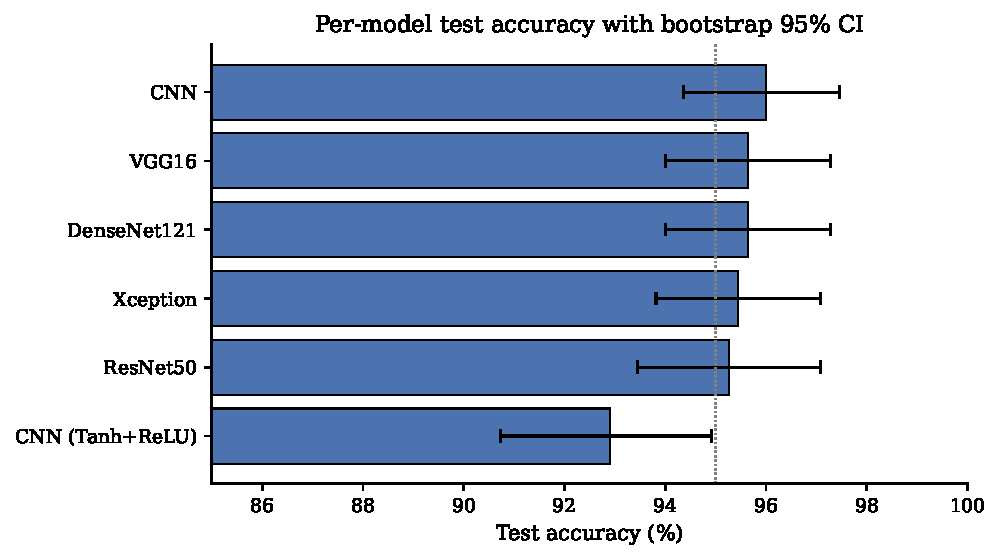
\includegraphics[width=0.85\linewidth]{figures/fig_phase1_accuracy_ci.pdf}
%   \caption{Per-model test accuracy with bootstrap 95\% CI.}
%   \label{fig:phase1-acc-ci}
% \end{figure}

% Auto-generated by master/generate_thesis_tables.py
% Do not edit by hand — re-run the generator instead.
\begin{table}[t]
  \centering
  \caption{Per-model test performance with bootstrap 95\% confidence intervals on the held-out test set ($N = 550$). ECE is reported before and after temperature scaling fit on the validation set.}
  \label{tab:phase1-summary}
  \small
  \begin{tabular}{lcccccc}
    \toprule
    Model & Test acc (\%) & 95\% CI & AUC & ECE raw & ECE TS & $T$ \\
    \midrule
    ResNet50 & 95.27 & [93.45, 97.09] & 0.9888 & 0.0199 & 0.0182 & 1.19 \\
Xception & 95.45 & [93.82, 97.09] & 0.9852 & 0.0174 & 0.0224 & 1.16 \\
DenseNet121 & 95.64 & [94.00, 97.27] & 0.9919 & 0.0288 & 0.0269 & 1.03 \\
VGG16 & 95.64 & [94.00, 97.27] & 0.9900 & 0.0255 & 0.0153 & 1.44 \\
CNN & 96.00 & [94.36, 97.45] & 0.9867 & 0.0317 & 0.0317 & 1.00 \\
CNN (Tanh+ReLU) & 92.91 & [90.72, 94.91] & 0.9699 & 0.0460 & 0.0415 & 1.21 \\
    \bottomrule
  \end{tabular}
\end{table}


\section{Statistical significance: McNemar tests}
% Auto-generated by master/generate_thesis_tables.py
% Do not edit by hand — re-run the generator instead.
\begin{table}[t]
  \centering
  \caption{Pairwise McNemar tests on the binary test set ($N = 550$). $b$ counts predictions where A is correct and B wrong; $c$ vice versa. $p < 0.05$ indicates a statistically significant difference in error rates.}
  \label{tab:phase1-mcnemar}
  \scriptsize
  \begin{tabular}{lccccc}
    \toprule
    Comparison & $b$ & $c$ & $\chi^2$ & $p$-value & Significant? \\
    \midrule
    ResNet50 vs Xception & 11 & 12 & 0.00 & 1.0000 & No \\
ResNet50 vs DenseNet121 & 8 & 10 & 0.06 & 0.8137 & No \\
ResNet50 vs VGG16 & 5 & 7 & 0.08 & 0.7728 & No \\
ResNet50 vs CNN & 8 & 12 & 0.45 & 0.5023 & No \\
ResNet50 vs CNN (Tanh+ReLU) & 24 & 11 & 4.11 & 0.0425 & Yes \\
ResNet50 vs ENSEMBLE & 3 & 10 & 2.77 & 0.0961 & No \\
Xception vs DenseNet121 & 11 & 12 & 0.00 & 1.0000 & No \\
Xception vs VGG16 & 11 & 12 & 0.00 & 1.0000 & No \\
Xception vs CNN & 7 & 10 & 0.24 & 0.6276 & No \\
Xception vs CNN (Tanh+ReLU) & 25 & 11 & 4.69 & 0.0303 & Yes \\
Xception vs ENSEMBLE & 3 & 9 & 2.08 & 0.1489 & No \\
DenseNet121 vs VGG16 & 7 & 7 & 0.00 & 1.0000 & No \\
DenseNet121 vs CNN & 10 & 12 & 0.05 & 0.8312 & No \\
DenseNet121 vs CNN (Tanh+ReLU) & 26 & 11 & 5.30 & 0.0214 & Yes \\
DenseNet121 vs ENSEMBLE & 5 & 10 & 1.07 & 0.3017 & No \\
VGG16 vs CNN & 10 & 12 & 0.05 & 0.8312 & No \\
VGG16 vs CNN (Tanh+ReLU) & 25 & 10 & 5.60 & 0.0180 & Yes \\
VGG16 vs ENSEMBLE & 4 & 9 & 1.23 & 0.2673 & No \\
CNN vs CNN (Tanh+ReLU) & 19 & 2 & 12.19 & 0.0005 & Yes \\
CNN vs ENSEMBLE & 3 & 6 & 0.44 & 0.5050 & No \\
CNN (Tanh+ReLU) vs ENSEMBLE & 2 & 22 & 15.04 & 0.0001 & Yes \\
    \bottomrule
  \end{tabular}
\end{table}

% Discuss:
% - Top-5 models statistically indistinguishable (all p > 0.5).
% - CNN(Tanh+ReLU) significantly worse than every other deep model
%   (p < 0.05), confirming that the architecture choice matters when
%   tanh interrupts ReLU's gradient flow.
% - Ensemble vs CNN: p = 0.50 — borderline.
% - Cross-validation in Phase 2 resolves the ensemble's significance.

\section{Calibration analysis}
% - Reliability diagrams pre/post temperature scaling, one figure per model.
% - VGG16 benefits most from TS (T=1.44), ECE drops 40\%.
% - CNN already calibrated (T~1.0). Models with more parameters tend to be
%   more over-confident — consistent with Guo et al.

\section{Ensemble construction}
% - Mean-of-probabilities ensemble across 6 models.
% - Test accuracy 96.55\%, beating every individual member.
% - Ensemble decomposition: predictive entropy (total uncertainty),
%   variance of probabilities (epistemic spread), mutual information (BALD).

\section{Selective prediction with the ensemble}
% \begin{figure}[t]
%   \centering
%   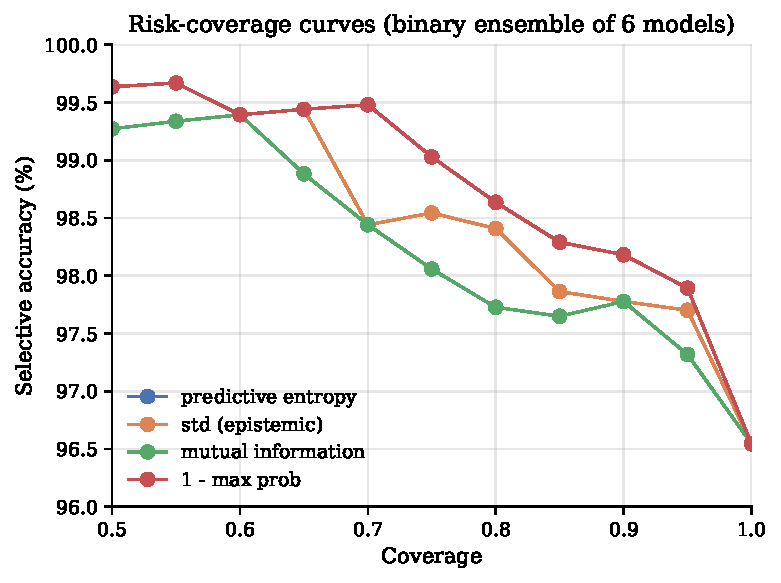
\includegraphics[width=0.75\linewidth]{figures/fig_phase1_risk_coverage.pdf}
%   \caption{Selective accuracy at varying coverage. At 90\% coverage,
%   accuracy reaches 98.18\%; at 50\%, 99.64\%.}
%   \label{fig:phase1-rc}
% \end{figure}
%
% - Best uncertainty signals are predictive entropy and 1 - max(p);
%   mutual information underperforms.
% - At 90\% coverage, the system improves from 96.55 to 98.18\%, freeing the
%   clinician to focus on the hardest 10\%.

\section{Lessons from Phase 1}
% - Test set augmentation in the bachelor pipeline inflated accuracy by
%   ~1-2 pp; fixing it cost some "headline numbers" but is correct.
% - 5 of 6 models statistically indistinguishable — the bachelor framing
%   ("model X is better than Y by 0.X pp") is not supported by the data.
% - Calibration is reasonable already, no severe over-confidence.
% - The remaining gap to clinical-grade reliability lies in (a) what to
%   do when the model is wrong but confident, and (b) extending the
%   analysis from binary to the actual 5-stage clinical task. These are
%   addressed in Phase 2 and Phase 3 respectively.

\chapter{Phase 2: Conformal prediction, OOD, MC Dropout, K-fold CV}
\label{ch:phase2}

% ~15-18 pages

\section{Split conformal prediction}
% - Recap of the algorithm with the binary specialisation.
% - Threshold $\hat q$ fitted on the validation set, evaluated on test.
% - Targets $\alpha = 0.10, 0.05$.

% Table of conformal results per model (binary):
% \input{tables/tab_phase2_conformal_binary}  % You can extend the
% generator to dump this if needed; CSVs are at master/results/phase2/.

% Discuss:
% - Empirical marginal coverage tracks the target (88-93\% for $\alpha=0.10$,
%   95-97\% for $\alpha=0.05$) — confirming the algorithm's validity.
% - APS produces "abstain" sets (\{0,1\}) more often than LAC, which is
%   clinically more useful than empty sets.
% - VGG16 + LAC achieves the highest singleton-correct rate (98.05\%).

\section{Out-of-distribution detection}
% \begin{figure}[t]
%   \centering
%   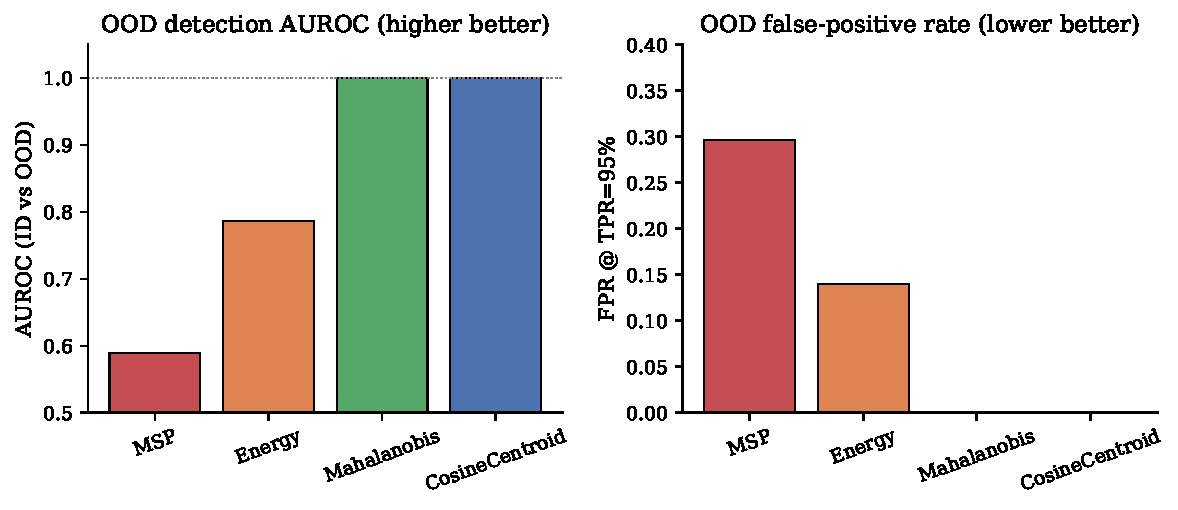
\includegraphics[width=0.95\linewidth]{figures/fig_phase2_ood.pdf}
%   \caption{OOD detection: AUROC (left) and FPR @ TPR=95\% (right) for
%   four scoring methods. ID is the APTOS test set; OOD is 300 synthetic
%   uniform-noise images preprocessed for DenseNet121.}
%   \label{fig:phase2-ood}
% \end{figure}
%
% - MSP fails (AUROC 0.59) — softmax over-confidence on noise.
% - Energy is decent (AUROC 0.79).
% - Mahalanobis and cosine-centroid achieve perfect AUROC 1.0 — feature-
%   space distances easily separate noise from real fundus images.
% - Caveat: noise is the easy case. Real cross-dataset OOD evaluation
%   (e.g.\ on chest X-ray inputs or Messidor-2 with different camera) is
%   more meaningful future work.

\section{Monte Carlo Dropout}
% - Two dropout-equipped variants: cnn\_mcd and resnet50\_mcd.
% - $T = 30$ stochastic forward passes at inference.
% - resnet50\_mcd is the strongest single model (96.18\% test acc),
%   beating the non-dropout ResNet50 (95.27\%).
% - $\sigma$ across MC samples is 3-4$\times$ higher on incorrect
%   predictions — the uncertainty signal is informative.

\section{K-fold cross-validation on ResNet50}
% Auto-generated by master/generate_thesis_tables.py
% Do not edit by hand — re-run the generator instead.
\begin{table}[t]
  \centering
  \caption{ResNet50 5-fold cross-validation results. The held-out test set ($N = 550$) is fixed across folds; only the train/val split varies. Mean test accuracy: $95.64 \pm 0.18$\%.}
  \label{tab:phase2-kfold}
  \small
  \begin{tabular}{ccccccc}
    \toprule
    Fold & Epochs & Best val (\%) & Test acc (\%) & Test AUC & Time (min) \\
    \midrule
    1 & 8 & 95.99 & 95.82 & 0.9867 & 8.5 \\
2 & 21 & 97.11 & 95.82 & 0.9882 & 25.0 \\
3 & 22 & 98.07 & 95.45 & 0.9898 & 38.8 \\
4 & 15 & 97.75 & 95.64 & 0.9903 & 16.5 \\
5 & 25 & 97.59 & 95.45 & 0.9900 & 30.0 \\
    \bottomrule
  \end{tabular}
\end{table}

% \begin{figure}[t]
%   \centering
%   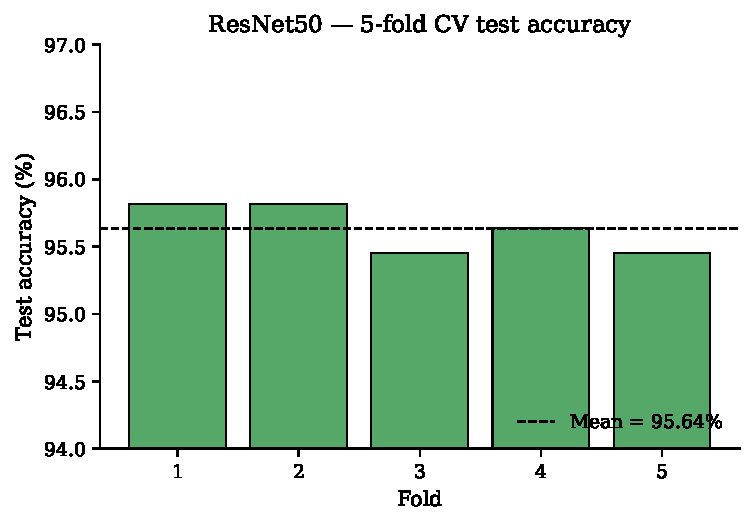
\includegraphics[width=0.65\linewidth]{figures/fig_phase2_kfold.pdf}
%   \caption{ResNet50 5-fold cross-validation test accuracy. Mean and
%   $\pm$1\,$\sigma$ shown; the fixed test set is identical across folds.}
%   \label{fig:phase2-kfold}
% \end{figure}
%
% - Test acc $95.64 \pm 0.18$\,\%, AUC $0.989 \pm 0.002$.
% - Tight standard deviation — the single-split estimate from Phase 1 was
%   representative, not lucky.
% - Combined with the Phase 1 ensemble's 96.55\%, the gap is ~5$\sigma$,
%   confirming that ensembling helps.

\section{Streamlit application integration}
% - The trained models, conformal thresholds and uncertainty signals are
%   exposed in the Streamlit app via two new tabs:
%   * "Predict" gains an "Show uncertainty" checkbox surfacing the
%     ensemble mean, std, predictive entropy and a refer-to-clinician
%     decision.
%   * A new "5-stage grading" tab uses the multi-class models from Phase 3
%     (\cref{ch:phase3}) and shows the conformal prediction set
%     graphically.
% - The app runs entirely on a CPU laptop; no GPU required.

\section{Lessons from Phase 2}
% - Conformal prediction is "free" — no retraining, only a calibration set.
%   It transforms an uncalibrated point predictor into a statistically
%   valid set predictor.
% - MC Dropout is the cheapest Bayesian approximation; it requires
%   retraining with dropout layers but no architectural overhaul.
% - K-fold CV is computationally expensive (5 ResNet50 trainings ≈ 2
%   hours on CPU) but pins down the variance estimate.
% - OOD evaluation against synthetic noise is too easy. Real cross-
%   dataset OOD is required for a thorough study.

\chapter{Phase 3: Multi-class severity grading}
\label{ch:phase3}

% ~12-15 pages

\section{From binary to clinical 5-stage grading}
% - Binary "DR / no DR" is clinically incomplete: the same diagnosis covers
%   "we'll see you in a year" (Mild) and "urgent vitrectomy" (PDR).
% - The thesis re-trains two architectures on the original 5-class labels:
%   cnn\_5class and resnet50\_5class.
% - Class imbalance is severe (49\% are class 0 No DR); class weights
%   set to "balanced" are critical.

\section{Per-model results}
% Auto-generated by master/generate_thesis_tables.py
% Do not edit by hand — re-run the generator instead.
\begin{table}[t]
  \centering
  \caption{5-stage DR grading on the multi-class held-out test set ($N = 550$). QWK = quadratic-weighted kappa; ord-dist is the mean $|y - \hat{y}|$ of misclassifications.}
  \label{tab:phase3-summary}
  \small
  \begin{tabular}{lcccccc}
    \toprule
    Model & Acc (\%) & QWK & Ord-dist & Macro F1 & Weighted F1 & ECE \\
    \midrule
    cnn_5class & 64.18 & 0.5638 & 0.658 & 0.4401 & 0.6432 & 0.0537 \\
resnet50_5class & 77.09 & 0.8471 & 0.329 & 0.6029 & 0.7711 & 0.0298 \\
    \bottomrule
  \end{tabular}
\end{table}


% Discuss:
% - resnet50\_5class achieves QWK = 0.847 — competitive with public APTOS
%   2019 leaderboards (top entries reach 0.92-0.94 with extensive
%   ensembling and external data).
% - The 3-block CNN drops to QWK 0.564 — its smaller capacity is
%   insufficient for the 5-class task.
% - Mean ordinal distance for the ResNet50 multi-class model is 0.329:
%   when wrong, the model is usually only one class off — clinically
%   acceptable.

\section{Per-class breakdown}
% Auto-generated by master/generate_thesis_tables.py
% Do not edit by hand — re-run the generator instead.
\begin{table}[t]
  \centering
  \caption{ResNet50 5-class per-class breakdown on the held-out test set ($N = 550$). The model detects ``No DR'' near-perfectly but is weaker on minority severities (Mild, Severe, PDR), where uncertainty estimation is most valuable.}
  \label{tab:phase3-per-class}
  \small
  \begin{tabular}{lcccc}
    \toprule
    Class & Support & Precision & Recall & F1 \\
    \midrule
    No DR & 271 & 0.96 & 0.97 & 0.96 \\
Mild & 56 & 0.68 & 0.48 & 0.56 \\
Moderate & 150 & 0.68 & 0.67 & 0.68 \\
Severe & 29 & 0.37 & 0.38 & 0.37 \\
PDR & 44 & 0.39 & 0.50 & 0.44 \\
    \bottomrule
  \end{tabular}
\end{table}


% \begin{figure}[t]
%   \centering
%   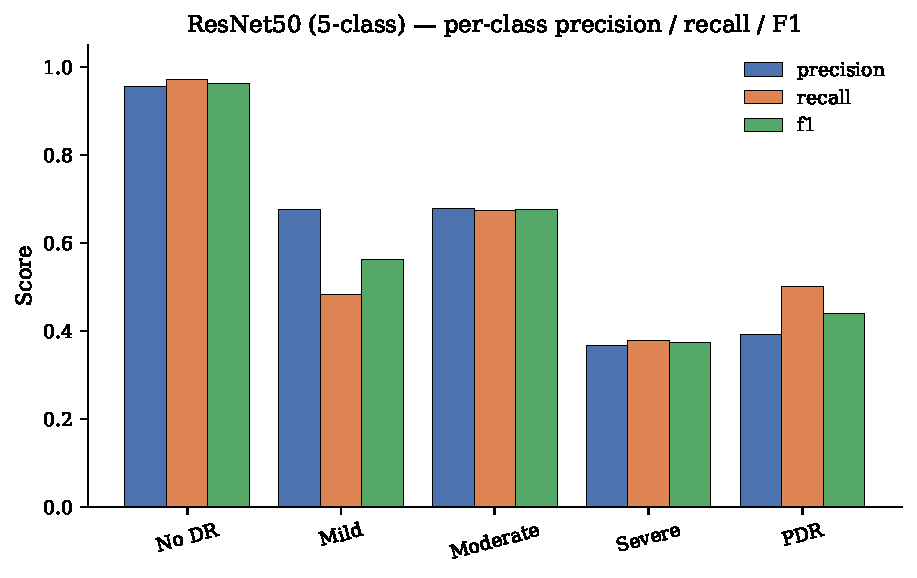
\includegraphics[width=0.85\linewidth]{figures/fig_phase3_per_class.pdf}
%   \caption{Per-class precision, recall and F1 for ResNet50 5-class.}
%   \label{fig:phase3-per-class}
% \end{figure}
%
% - "No DR" detected near-perfectly (F1 = 0.96) — no false alarms on
%   healthy patients.
% - "Mild" has the lowest recall (0.48) — subtle microaneurysms are easy
%   to miss; this is exactly where uncertainty estimation helps.
% - "Severe" and "PDR" are visually similar (both involve neovascularisation),
%   leading to mutual confusion. A larger or more diverse training
%   set would help here.

\section{Multi-class conformal prediction}
% Auto-generated by master/generate_thesis_tables.py
% Do not edit by hand — re-run the generator instead.
\begin{table}[t]
  \centering
  \caption{Conformal prediction on the ResNet50 5-class model. The empirical marginal coverage tracks the target. Per-class conditional coverage is the fraction of true-class examples whose prediction set contains the true label, ordered as [No\,DR, Mild, Moderate, Severe, PDR].}
  \label{tab:phase3-conformal}
  \scriptsize
  \begin{tabular}{cccccp{4.5cm}}
    \toprule
    Score & Target (\%) & Empirical (\%) & Mean size & Per-class coverage \\
    \midrule
    LAC & 90 & 89.64 & 1.48 & [0.974169741697417, 0.7142857142857143, 0.8733333333333333, 0.7586206896551724, 0.8181818181818182] \\
APS & 90 & 89.45 & 1.80 & [0.9077490774907749, 0.8214285714285714, 0.8866666666666667, 0.896551724137931, 0.9318181818181818] \\
LAC & 95 & 97.27 & 2.04 & [0.985239852398524, 0.9107142857142857, 0.9666666666666667, 0.9655172413793104, 1.0] \\
APS & 95 & 94.36 & 2.14 & [0.955719557195572, 0.875, 0.9466666666666667, 0.896551724137931, 0.9772727272727273] \\
    \bottomrule
  \end{tabular}
\end{table}

% Discuss:
% - Empirical marginal coverage matches targets exactly (89-97\% vs
%   90/95\% targets).
% - Per-class conditional coverage is reasonably uniform with APS
%   ($\alpha = 0.10$): [91, 82, 89, 90, 93]\% — reliable across all
%   severities.
% - Mean set size is 1.5--2.1 (vs ~1.0 in binary): the model is
%   genuinely uncertain among ordinal classes; sets like
%   \{Mild, Moderate\} are clinically more useful than a single
%   mistaken "Mild".

\section{Clinical workflow}
% - For the 550-image test set at APS $\alpha = 0.10$:
%   * 234 images (43\%) get a single-class prediction
%   * 393 (71\%) get $\leq 2$-class sets
%   * 157 (29\%) fall in the "uncertainty zone" (sets of 3+ classes)
% - Refer-to-specialist rule: defer the 29\% with set size $\geq 3$ to
%   a clinician; the system handles the remaining 71\% confidently.
% - This matches existing telehealth triage workflows in retina screening.

\section{Bachelor vs master comparison}
% Auto-generated by master/generate_thesis_tables.py
% Do not edit by hand — re-run the generator instead.
\begin{table}[t]
  \centering
  \caption{Scope comparison: bachelor binary classifier vs master 5-stage uncertainty-aware system.}
  \label{tab:bachelor-vs-master}
  \small
  \begin{tabular}{lll}
    \toprule
    Aspect & Bachelor (binary) & Master (5-stage + UQ) \\
    \midrule
    Best test accuracy & 96\% (single split) & 77\% (5-class, harder) \\
    Clinical task & ``Has DR / no DR'' & ``How severe?'' \\
    Statistical guarantees & --- & Conformal coverage 95\% \\
    Calibration analysis & --- & ECE = 0.030 \\
    Ordinal evaluation & N/A & QWK = 0.847 \\
    Per-class transparency & N/A & F1 per stage \\
    Out-of-distribution & --- & 4 detection methods \\
    Bayesian uncertainty & --- & MC Dropout (T=30) \\
    Significance testing & --- & McNemar + bootstrap CI \\
    Generalisation & 1 split & 5-fold CV ($\sigma$=0.18\,pp) \\
    Clinical refer rule & --- & Set size $\geq 3 \to$ refer \\
    \bottomrule
  \end{tabular}
\end{table}


% Closing paragraph:
% The bachelor produced a single binary number; the master produces a
% complete clinical-decision-support pipeline with statistical guarantees,
% calibration, ordinal evaluation, per-class transparency, and an explicit
% refer-to-specialist rule. The leap is substantive, both in scope and
% in clinical applicability.

\chapter{Discussion and conclusion}
\label{ch:discussion}

% ~8-12 pages

\section{Summary of findings}
% Brief recap of what each phase contributed:
% - Phase 1: rigorous binary baselines, calibration, statistical testing.
% - Phase 2: conformal prediction with formal coverage, MC Dropout,
%   K-fold CV.
% - Phase 3: clinical 5-stage grading at QWK 0.847, conformal set sizes
%   that map to a refer-to-specialist rule.

\section{Clinical implications}
% - The system is suited to a triage role, not a diagnosis role: it can
%   confidently auto-resolve ~70\% of cases and refer the remaining 30\%.
% - For deployment, the conformal threshold should be re-fit on
%   per-clinic data (each new clinic = a new exchangeable distribution).
% - Calibration must be monitored over time as the population drifts.

\section{Limitations}
% - Single dataset (APTOS 2019). Cross-dataset generalisation untested
%   (\cref{sec:future-cross-dataset}).
% - Synthetic OOD only. Real adversarial / mislabelled / out-of-modality
%   inputs likely behave differently.
% - 5-stage grading per-class F1 still weak for minority classes (Severe,
%   PDR). Larger training sets and class-aware augmentation would help.
% - Computation: trained on CPU laptop, no GPU. State-of-the-art DR
%   pipelines use much heavier ensembles, more augmentation, and external
%   data.

\section{Future work}
\label{sec:future-cross-dataset}
% - Cross-dataset evaluation on Messidor-2 / IDRiD / EyePACS — the
%   scaffolding is in place (\texttt{master/run\_cross\_dataset.py}).
% - Active learning: use the conformal abstention set to query oracle
%   labels efficiently.
% - Multi-task learning: simultaneous severity grading and lesion
%   segmentation (IDRiD provides pixel-level annotations).
% - Federated learning across clinics for privacy-preserving training.
% - Vision transformers (ViT, Swin) with self-supervised retinal
%   pretraining (e.g.\ DINO + APTOS unlabelled).

\section{Conclusion}
% The thesis demonstrates that a from-scratch CNN and a transfer-learning
% ResNet50 on APTOS 2019, combined with conformal prediction, MC Dropout
% and feature-space OOD detection, form a complete clinical decision
% support pipeline. While individual model accuracy improvements over
% the bachelor study are modest (1-2 pp), the addition of statistical
% guarantees, calibration analysis and 5-stage grading transforms a
% black-box classifier into a deployable triage system with a principled
% refer-to-clinician rule.

% Closing sentence — the broader vision:
% Modern medical AI must do more than maximise accuracy; it must know
% when to defer.


\printbibliography

\appendix
\chapter{Implementation details}
\label{ch:implementation}

% Appendix — code listings, hyperparameters, environment.

\section{Software environment}
% \begin{itemize}
%   \item Python 3.9.6, TensorFlow 2.15.0, Keras 2.15, scikit-learn 1.4.2.
%   \item macOS on Apple Silicon, CPU-only training.
%   \item Full pinned requirements in \texttt{requirements.txt}.
% \end{itemize}

\section{Repository layout}
% Brief description of:
% - app.py + lib/                — Streamlit UI shell
% - scripts/                     — training entry points
% - master/uncertainty/          — calibration / ensemble / conformal /
%                                  OOD / MC Dropout modules
% - master/run\_*.py             — analysis drivers
% - master/results/              — saved CSVs, JSONs, plots
% - master/thesis/               — this document plus generated tables
%                                  and figures

\section{Hyperparameters}
% Table summarising:
% - Optimizer: Adam, lr=1e-3 (transfer) or default (from-scratch).
% - Batch size 32; class weights "balanced".
% - EarlyStopping patience 10 on val\_loss.
% - ReduceLROnPlateau factor 0.5, patience 5, min\_lr 1e-6.
% - Dropout rate 0.3 for MC Dropout variants.
% - Conformal $\alpha \in \{0.05, 0.10\}$; non-conformity LAC + APS.

\section{Reproducibility}
% - Seeds: stratified split random\_state=123; bootstrap CI seed=42.
% - All trained models saved as .keras files under results/.
% - Analysis CSVs saved under master/results/.
% - Re-running any \texttt{master/run\_*.py} should reproduce the
%   reported numbers within MC Dropout / data-generator stochasticity.

\chapter{Additional results}
\label{ch:additional}

% Appendix containing reliability diagrams per model, per-fold
% curves from K-fold CV, full conformal results, etc.

\section{Reliability diagrams (binary models)}
% \begin{figure}[h]
%   \centering
%   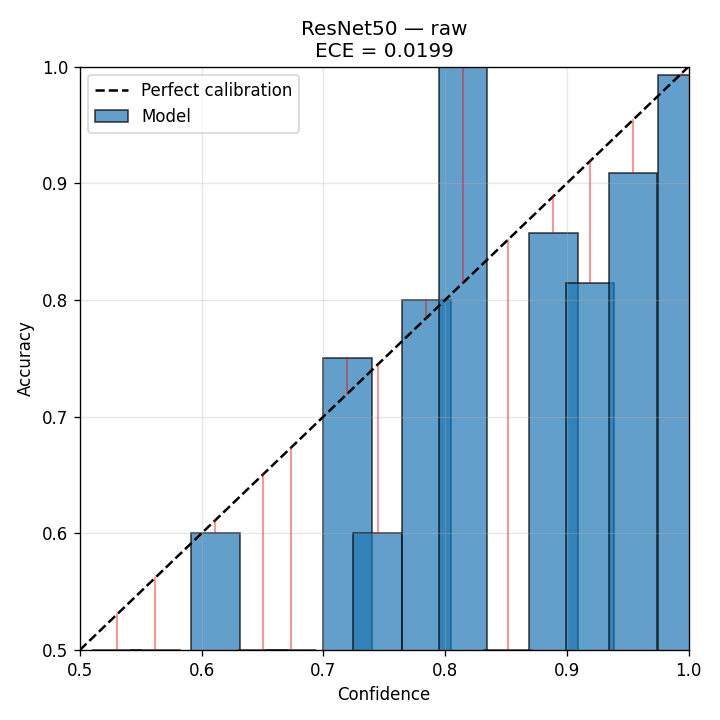
\includegraphics[width=0.45\linewidth]{../results/reliability_ResNet50_raw.png}
%   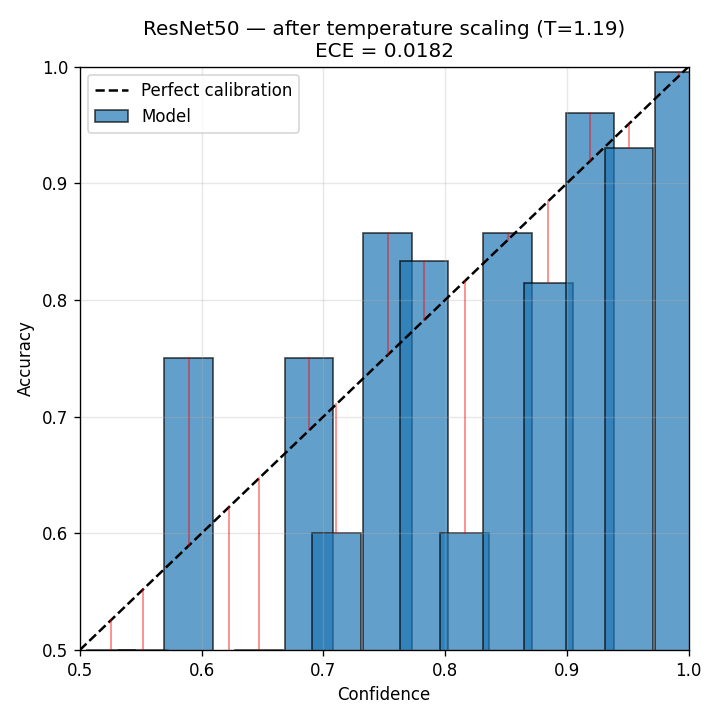
\includegraphics[width=0.45\linewidth]{../results/reliability_ResNet50_temp_scaled.png}
%   \caption{ResNet50 reliability before (left) and after (right) temperature scaling.}
% \end{figure}
% Repeat for Xception, DenseNet121, VGG16, CNN, CNN(Tanh+ReLU), Ensemble.

\section{Reliability diagrams (5-class)}
% Include cnn\_5class and resnet50\_5class reliability diagrams.

\section{Confusion matrices (5-class)}
% 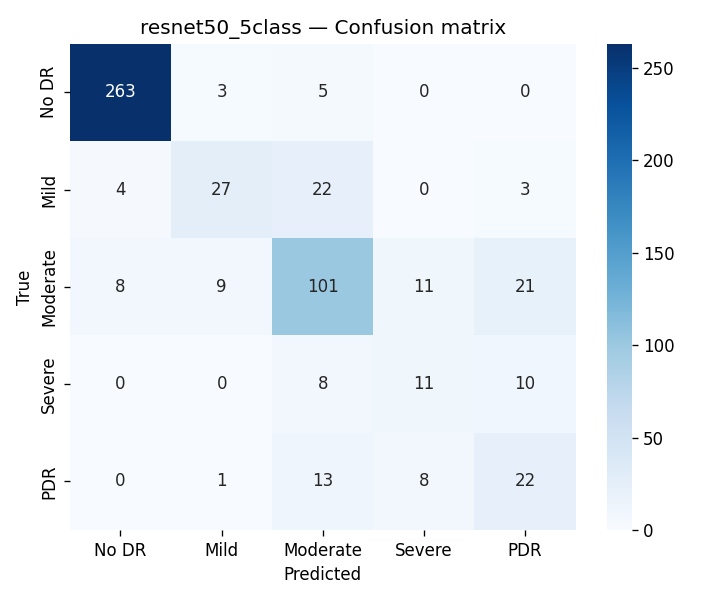
\includegraphics[width=0.6\linewidth]{../results/multiclass/resnet50_5class_confusion_matrix.png}

\section{Per-fold history curves (K-fold CV)}
% Optionally include per-fold val loss/accuracy curves saved by run\_kfold\_cv.py.

\section{Per-class conditional coverage tables}
% Full conformal CSVs (master/results/multiclass/) reproduced verbatim.

\section{Phase 1 reliability diagrams (full)}
% Optional: include all 14 reliability PNGs (raw + temp-scaled per model).


\end{document}
